\documentclass[a4paper,11pt,cours]{nsi} % COMPILE WITH DRAFT
\geometry{margin=2cm}
\usepackage{hyperref}
\usepackage{yhmath}

\begin{document}

\setcounter{chapter}{6} % 1 de moins que le num de chapitre



\chapter{Trigonométrie}


\setlength{\columnseprule}{0.5pt}
\setlength{\columnsep}{1cm}

Dans le plan, on choisit une \emph{orientation} : on décide de manière arbitraire que le \emph{sens direct} est le sens de 
rotation contraire à celui des aiguilles d'une montre. L'autre sens et appelé \emph{sens indirect}.
\begin{center}
	\begin{tikzpicture}
		\draw[UGLiOrange,very thick,->](0,1)  arc (20:340:1);
		\draw (-1,-.5) node[below]{sens direct};
	\end{tikzpicture}
	\hspace*{2cm}
	\begin{tikzpicture}
		\draw[UGLiOrange,very thick,<-](0,1)  arc (20:340:1);
		\draw (-1,-.5) node[below]{sens indirect};
	\end{tikzpicture}
\end{center}

\section{\boldmath\textbf{L'enroulement de R sur le cercle trigonométrique}}
\begin{minipage}{7cm}
	\begin{tikzpicture}[scale = 2]
		\reperev{-1.5}{-1.5}{1.5}{3}
		\draw[thick,UGLiOrange] (0,0) circle (1cm);
		\draw[UGLiDarkBlue] (1,-1.5)-- (1,2);
		\draw (1,0)\ball node[below right]{I} (1,1) \ball node[right]{$1$};
		\draw [->,>=stealth, very thick](1,0)-- (1,3);
		\draw[very thick](1,0)--(1,2.75)\ball node(G){}node[right]{$x$};	
		\draw[very thick] (1,0) arc (0:57.3*2.75:1)\ball node (H){} node[above left]{$M(x)$};
		\draw[thick,dashed,green!40!black,->,bend right] (G) to (H.north);
		\draw[very thick](1,0)--(1,-1.25)\ball node(E){};
		\draw[very thick] (1,0) arc (0:-57.3*1.25:1)\ball node (F){};
		\draw[thick,dashed,green!40!black,->,bend left] (E) to (F);
		\draw[very thick](1,0)--(1,1.5)\ball node(C){};
		\draw[very thick] (1,0) arc (0:57.3*1.5:1)\ball node (D){};
		\draw[thick,dashed,green!40!black,->,bend right] (C) to (D);
		\draw[very thick](1,0)--(1,1)\ball node(A){};
		\draw[very thick] (1,0) arc (0:57.3:1)\ball node[below] (B){$M(1)$};
		\draw[thick,dashed,green!40!black,->,bend right] (A) to (B);
		\draw(-.7,-.9) node{$\mathcal{C}$};
        \draw(1,3) node[below left]{$(\mathcal{D})$};
	\end{tikzpicture}
\end{minipage}
\begin{minipage}{10cm}
	Un cercle trigonométrique est un cercle de rayon 1. Il est fréquent de munir le plan d'un repère orthonormal $\rep$ et de prendre pour cercle 
	trigonométrique le cercle $\mathcal{C}$ de rayon 1 centré en O.\\
	
	%Dans ce repère on  considère les points $\pc{I}{1}{0}$ et $\pc{A}{1}{1}$. 
    Soit $(\mathcal{D})$ la droite passant par $\pc{I}{1}{0}$, orientée et dirigée par $\vv{j}$. La droite graduée $(\mathcal{D})$ représente alors l'ensemble $\R$.\\
    %I représente 0, A représente 1, et c\ae tera.\\
	
	On « enroule » $\R$ sur le cercle en faisant correspondre:
	\begin{enumerate}[label=\textbullet]
		\item 	zéro avec $I$;
		\item 	chaque point de $(\mathcal{D})$ représentant un réel positif $x$ avec l'unique point $M(x)$ du cercle tel que l'arc $
		\wideparen{IM}$ soit 
		\textbf{direct} et de 
		longueur 
		$x$;
		\item 	chaque point de $(\mathcal{D})$ représentant un réel négatif $x$ avec l'unique point $M(x)$ du cercle tel que l'arc $\wideparen{IM}$ soit l'image de $x$ sur 
		$\mathcal{C}$ et de longueur 
		$-x$.	
	\end{enumerate} 
	On appelle ce point $M(x)$ {\boldmath\textbf{l'image de $x$ sur $\mathcal{C}$}}.
\end{minipage}

\begin{propriete}[]
    Le cercle trigonométrique a pour longueur $2\pi$.
\end{propriete}
\begin{propriete}[]
	\begin{enumerate}[label=\textbullet]
		\item 	Deux nombres réels $x$ et $x'$ ont la même image sur $\mathcal{C}$ si et seulement si ces deux nombres sont séparés par un multiple 
		entier 
		de $2\pi$, 
		ce qui peut s'écrire {\boldmath $$x-x'=k\times2\pi\qquad(k\in\Z)$$}
		\item 	Si M est l'image d'un réel $x$ alors les nombres qui ont également $M$ pour image sont les réels de la forme 
		{\boldmath $$x+k\times2\pi\qquad(k\in \Z)$$}
	\end{enumerate}
\end{propriete}

%\begin{exemple}[s]
%    \carreauxseyes{16}{3.2}
%\end{exemple}

\begin{definition}[ : radian]
	\begin{minipage}{5cm}
		\begin{tikzpicture}[scale = 2]
			\draw(1.2,1.2)node{};
			\draw[thick] (0,0) circle (1cm);
			\draw[very thick,UGLiOrange] (1,0) arc (0:57.3:1) node[above right] (B){$M(1)$};
			\draw[very thick,UGLiOrange](0,0)--(57.3:1);
			\draw[very thick,UGLiOrange](0,0)--(1,0);
			\draw(0,0) node[below left]{O};
			\draw[very thick,UGLiOrange] (.3,0) arc (0:57.3:.3);
			\draw[UGLiOrange](1,.5)node{1};
			\draw[UGLiOrange](.5,.3)node{1 rad};	
			\draw(-.7,.9) node{$\mathcal{C}$};	
		\end{tikzpicture}
	\end{minipage}
	\begin{minipage}{11.5cm}
		On définit l'unité {\boldmath\textbf{ radian}} comme ceci : un radian est la mesure d'un angle qui intercepte un arc de $\mathcal{C}$ de longueur 1.\\
		\boldmath\textbf{360 degrés correspondent à $2\pi$ radians.}
	\end{minipage}
	
\end{definition}

\begin{propriete}[ : Conversion des mesures d'angles usuelles]
    \renewcommand{\arraystretch}{2}
    \tabstyle[UGLiRed]
    \begin{tabular}{|c|c|c|c|c|c|}
        \hline
        \ccell Angle (en degrés) & 360 & 180 & 90 & $d$ & $r\times \dfrac{360}{2\pi}$\\ \hline
        \ccell Angle (en radians) & $2\pi$ & $\pi$ & $\dfrac{\pi}{2}$ & $d\times \dfrac{2\pi}{360}$ & $r$ \\ \hline

    \end{tabular}
\end{propriete}

\begin{exemple}[s]
    \begin{enumerate}[label=\textbullet]
		\item 	Un angle de 30° mesure \dotfill radians.
		\item 	Un angle de 45° mesure \dotfill radians.
		\item 	Un angle de $\dfrac{\pi}{3}$ radians mesure \dotfill degrés.
		\item 	Un angle de $\dfrac{3\pi}{4}$ radians mesure \dotfill degrés.
	\end{enumerate}
\end{exemple}

\newpage



\section{Cosinus et sinus d'un nombre réel}

\dleft{10cm}{
	\begin{definition}[ : cosinus et sinus d'un nombre réel]
		Soit $x\in\R$. Soit $M$ son image sur $\mathcal{C}$.\\
		On appelle {\boldmath\textbf{cosinus de $x$}} et on note $\cos x$ l'abscisse de $M$.\\
		L'ordonnée de $M$ est le {\boldmath\textbf{sinus de $x$}}, noté $\sin x$.
	\end{definition}}
	{
		\begin{tikzpicture}[scale = 1.8]
			\draw[white,fill=white](-1.5,-1.5) rectangle (1.5,1.5);
			\reperea{-1.5}{-1.5}{1.5}{1.5}
			\draw(1.2,1.2)node{};
			\draw[thick] (0,0) circle (1cm);
			\draw(-.7,.9) node{$\mathcal{C}$};	
			\pointc{.6}{.8}{$\cos x$}{$\sin x$}{$M(x)$}
            \draw[UGLiOrange] (0,0) -- (.6,0.8);
            \draw[very thick,UGLiOrange] (.3,0) arc (0:54:.3) node[right] {$x$ rad};
	\end{tikzpicture}}


\begin{propriete}[s]
	
	Pour tout $x\in\R$ et pour tout $k\in\Z$ on a :
	\begin{enumerate}[label=\textbullet]
		\item 	{\boldmath\textbf{$-1\leqslant \cos x \leqslant 1$ et $-1\leqslant \sin x \leqslant 1$}}
		\item 	{\boldmath\textbf{$\cos\left(x+k\times2\pi\right)=\cos x	$ et $\sin\left(x+k\times2\pi\right)=\sin x$}}
		\item 	{\boldmath\textbf{$\cos^2x+\sin^2x=1$}}
	\end{enumerate}
\end{propriete}

%\begin{demonstration}
%    \carreauxseyes{16}{10.4}
%\end{demonstration}

\subsection*{Cosinus et sinus classiques}
\begin{center}
	\renewcommand{\arraystretch}{2.2}
    \tabstyle[UGLiOrange]
	\begin{tabular}{|c|c|c|c|c|c|c|}
		\hline 
		\ccell $x$ en degrés & $\quad 0\quad $&$\quad 30\quad$ &$\quad 45\quad $&$\quad 60\quad$ &$\quad 90\quad$ &$\quad 180\quad$ \\ 
		\hline 
		\ccell $x$ en radians & $0$ & $\dfrac{\pi}{6}$ & $\dfrac{\pi}{4}$ & $\dfrac{\pi}{3}$ & $\dfrac{\pi}{2}$ & $\pi$ \\ 
		\hline 
		\ccell $\cos x$ & $1$ & $\dfrac{\sqrt{3}}{2}$ & $\dfrac{\sqrt{2}}{2}$ & $\dfrac{1}{2}$ & 0 & $-1$ \\ 
		\hline 
		\ccell $\sin x$ & 0 & $\dfrac{1}{2}$ & $\dfrac{\sqrt{2}}{2}$ & $\dfrac{\sqrt{3}}{2}$ & $1$ & $0$ \\ 
		\hline 
	\end{tabular} 
\end{center}

\begin{demonstration}
	Démonstrations en vidéo : 
	\begin{enumerate}[label=\textbullet]
		\item 	Démontrer que $\sin\dfrac{\pi}{4}=\dfrac{\sqrt{2}}{2}$ : \href{ https://youtu.be/ViDEbKPzd34}{https://youtu.be/ViDEbKPzd34}
		\item Démontrer que $\sin\dfrac{\pi}{3}=\dfrac{\sqrt{3}}{2}$ et que $\cos\dfrac{\pi}{3}=\dfrac{1}{2}$ :	\href{https://youtu.be/gYeR0TzOHAw}{https://youtu.be/gYeR0TzOHAw}	
	\end{enumerate}
\end{demonstration}

\begin{center}
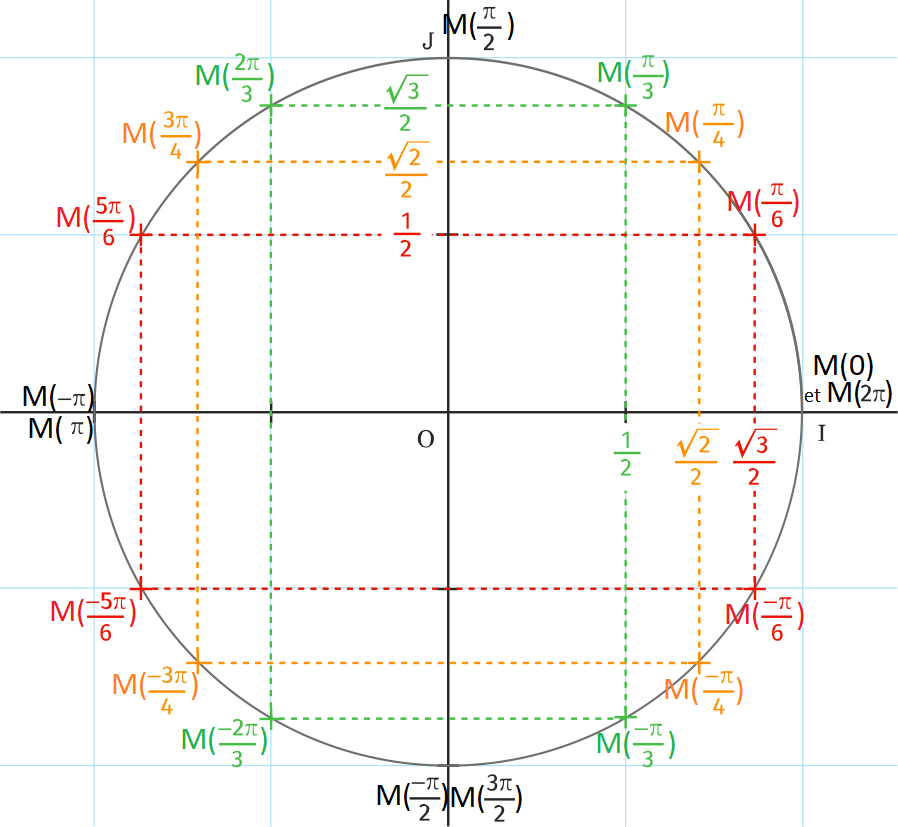
\includegraphics[width=14cm]{cercletrigo}
\end{center}



\begin{aretenir}
	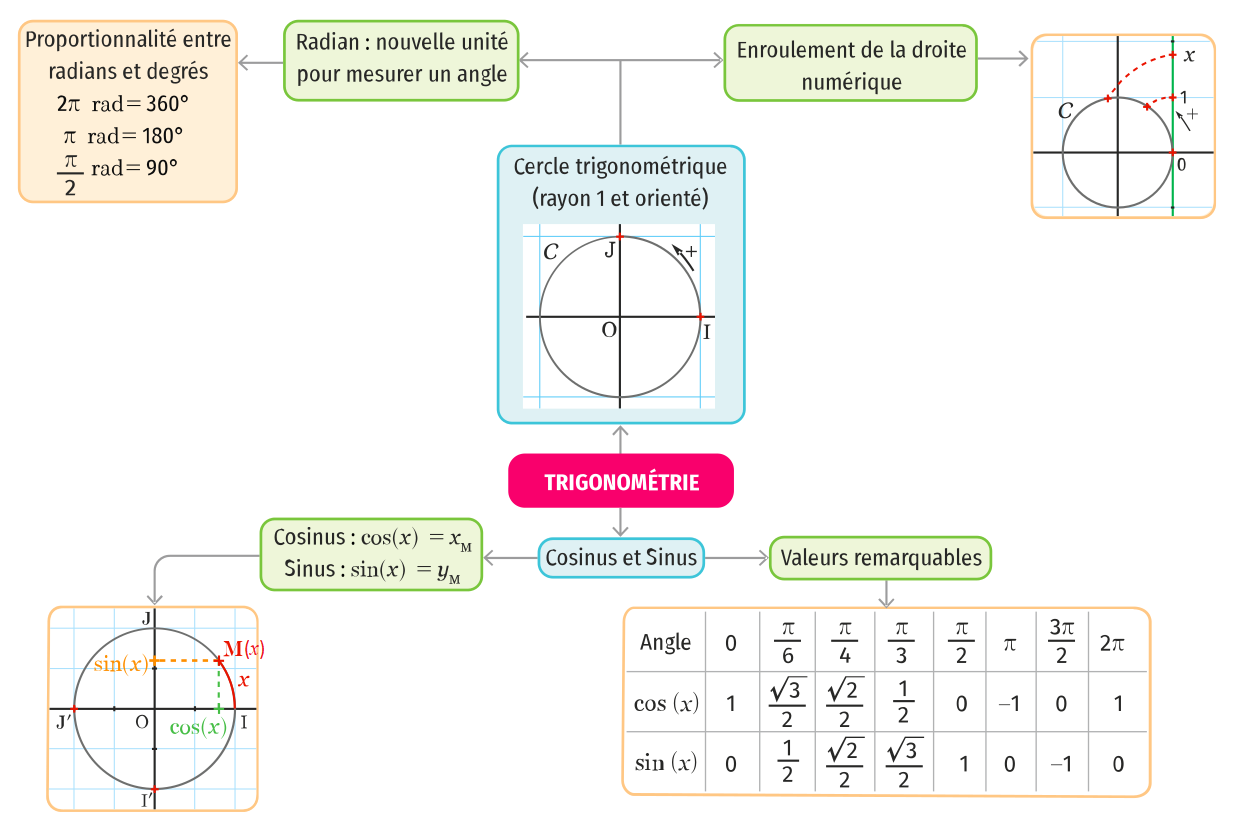
\includegraphics[width=16cm]{cartementale}
\end{aretenir}




\end{document}
